\documentclass{article}
\usepackage{graphicx}
\usepackage{authblk}
\usepackage{amsmath}


\begin{document}
\title{THEORETICAL NEUROSCIENCE \\ EXERCISE 3}
\date{\today}
\author[1]{\c{S}eyma Bayrak\thanks{seyma.bayrak@st.ovgu.de}}
\affil[1]{\footnotesize  Otto von Guericke University of Magdeburg}
\maketitle


\section*{Part 1}
The purpose of this exercise is to provide an imaginary step-functioned current, $i_{e}$, to the neuron, and then to analyze the behavior of membrane voltage, $V_{m}$.The whole electrical activity of neuron is thought to be a parallel connected circuit with resistor and capacitor elements. This assumption leads us to use ``Single Compartment Model -SCM'', which basically models $V_{m}$, with the already known value of input current and time range. The input current is modelled as given by equation 1.

\begin{equation}
 i_{e}=0,\,\,\,\,\,  0\le t <\dfrac{T}{4} \,\,\,and\,\,\, i_{e}=i_{0},\,\,\,\, \frac{3T}{4}<t\le T
\end{equation}

The step functioned current amplitude is $i_{e}$ is given as 12 $nA/\sqrt{mm}$, the current per unit membrane area, the total time range is between 0 and 500 $ms$. Subsequent to the modeling of input current and time vectors, the Euler’s simple integration method is programmed to find out membrane potential. A brief mathematical introduction of Euler’s Method is provided as the following,

\begin{equation}
 \dfrac{dV_{m}}{dt}=\dfrac{1}{\tau_{m}}[V_{\infty}(t)-V_{m}(t)] \,\, \longrightarrow \,\, dV_{m}=\dfrac{1}{\tau_{m}}[V_{\infty}(t)-V_{m}(t)].dt
\end{equation}

\begin{equation}
V_{m}(t+dt)=V_{m}(t)+dV_{m}
\end{equation}

where $\tau_{m}$ denotes so called ``time constant'', equivalent to the multiplication of resistivity and capacitance, both per unit membrane area, $\tau_{m}=r_{m}.c_{m}$. The equilibrium potential $V_{\infty}$ is defined in this exercise as the reversal potential $E_{L}$ added to classical Ohm`s Law potential, $V_{\infty}=r_{m}i_{e}(t)$. 

\begin{equation*}
r_{m}=1.5 M \Omega mm^{2}\,\,\,\,\,c_{m}=20nF/mm^{2}\,\,\,\,\,E_{L}=-65mV
\end{equation*}

\begin{center}
 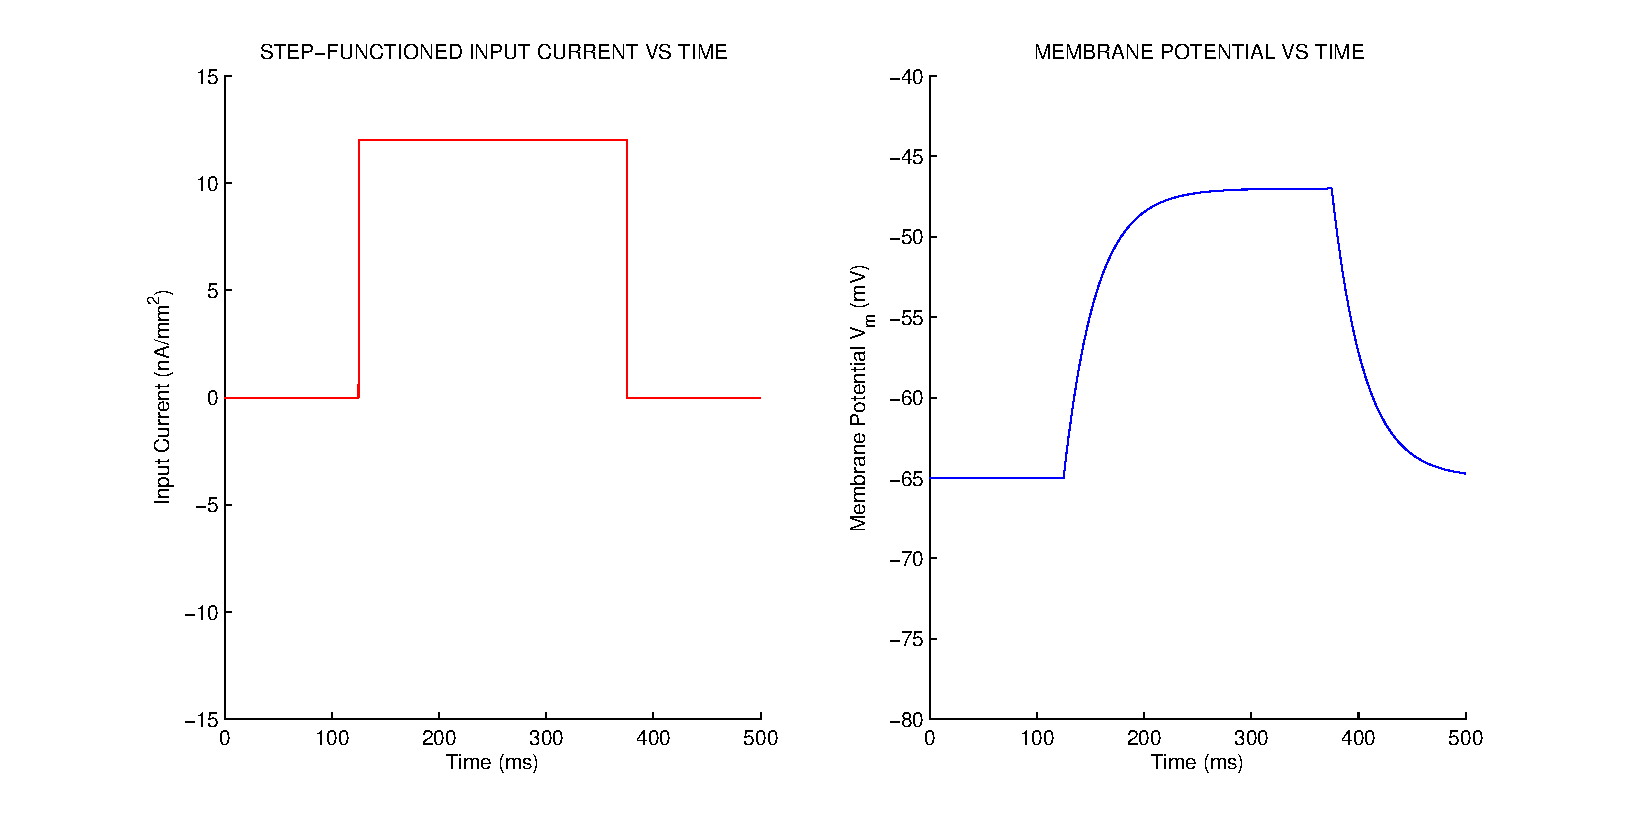
\includegraphics[width=\textwidth,  bb=0   231   682   610]{Exercise3/q7.eps}
 % q7.eps: 0x0 pixel, 300dpi, 0.00x0.00 cm, bb=  -86   231   682   610
Graph 1, The analysis of membrane potential caused by a step functioned input current, $V_{m}$ reaches to the maximum value of -47 mV, which is equals to the $V_{\infty}$ as expected.
\end{center}


\section*{Part 2}
The second part of exercise is much more interesting, now the imaginary action potentials are also taken into account, and we are even more close to the reality. Whenever the $V_{m}$ value equals to or exceeds the thereshold potential $V_{th}$, it suddenly falls down to level of reset potential $V_{reset}$. Therefore, $V_{m}$ is expected to have some ``spikes'' at the times on which the action potential occurs.





\end{document}






